%--------Preliminares
%--------Emir Muñoz Jiménez
%--------13-10-2010

\chapter{Marco Te\'orico}
\label{cap:preliminares}

\section{Impresión 3D}

 A diferencia de las técnicas principales que se emplean desde hace algunos años en la fabricación de objetos, que se encargan de sustraer, combinar, o deformar paulatina y controladamente materia hasta llegar a una pieza final, la impresión 3D funciona de un modo completamente distinto. La pieza se crea en un solo paso, capa por capa, a un ritmo medio de uno a dos centímetro de altura por hora; el objeto creado puede constar de mecanismos internos (como rodamientos de bolas), formas tejidas y entrelazadas, o incluso huecos y curvas \citep{Berchon2014}. Pues bien, todas las impresoras 3D, están basadas sobre el mismo principio: un modelo digital es transformado a un objeto físico de 3 dimensiones por adición de material en capas. Esto se conoce alternativamente como \textit{Manufactura Aditiva} \citep{tresdhub2018}. Este tipo de fabricación también se puede englobar dentro de lo que se denomina \textit{Fabricación digital}, cuyo principio básico es la transformación de la información  desde el mundo físico al digital. Según \citep{jorquera2016}, la fabricación digital incluye los siguientes sistemas y tecnologías:\\
 
 \begin{enumerate}
 	
	\item Sistemas integrados: Es un \textit{hardware} electrónico diseñado específicamente para llevar a cabo una o pocas tareas definidas. Las impresoras llevan un sistema electrónico integrado que utilizan para controlar los motores paso a paso que alimentan el papel, recibir información de los sensores de temperatura y finales de carrera, o que mandan al cabezal de impresión.
	\item Sistemas CNC (\textit{Computer Numeric Control} - control numérico computarizado): Es el control numérico de un sistema de automatización que se utiliza para controlar diferentes máquinas herramienta. Este sistema ha revolucionado la industria gracias a la simplificación del \textit{software} de diseño en conjunto con los lenguajes de programación como el \textit{.gcode}. Esencialmente, un sistema CNC es cualquier sistema que utiliza un ordenador para controlar los movimientos de una máquina.
	\item Software CAD (\textit{Computer Aided Design}- diseño asistido por computador): es, en esencia, un programa que sirve para la creación, edición análisis y visualización de modelos tridimensionales.  
	\item Internet: Los programas CAD actuales disponen de herramientas de trabajo colaborativo en red, de esta manera se define el producto y el proceso de fabricación de forma simultánea.\\

  \end{enumerate}

En la misma línea, y dependiendo de la profundidad técnica que el proceso de fabricación necesite, se agregan los sistemas \citep{leao2017}:

\begin{enumerate}
	\item Software CAE (\textit{Computer Aided Engineering} - Ingeniería Asistida por computador): Son los programas mayoritariamente usados para las tareas de análisis de ingeniería. Estos \textit{softwares}, a través de métodos numéricos como el método de elementos finitos o dinámica de fluidos computacional, se utilizan para, por ejemplo, analizar la robustez y el funcionamiento de ensambles de piezas.
	\item Software CAM (\textit{Computer Aided Manufacturing}- Manufactura Asistida por computador): Corresponde a programas que controlan las herramientas de máquinas de control numérico relacionadas con el proceso de manufactura a realizar, generando un código específico para el producto a fabricar. 

\end{enumerate}

%Figura: Expectativas impresi\'on 3D 
\begin{figure}[tp]
  \centering
    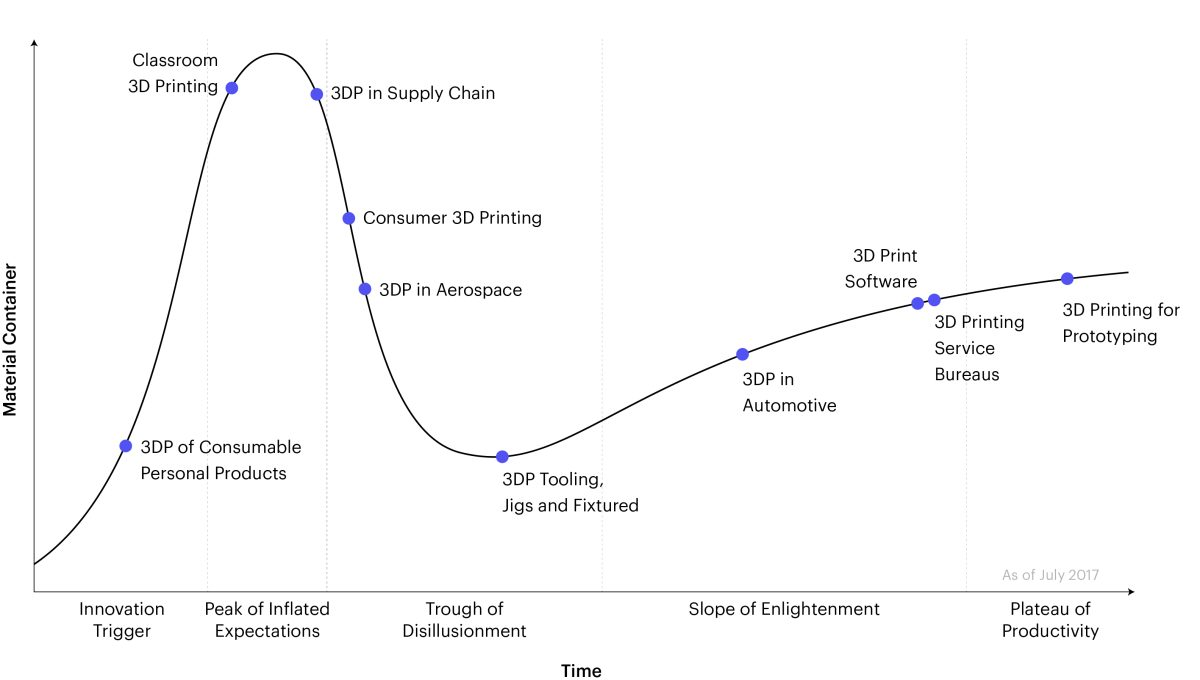
\includegraphics[width=\textwidth]{images/The3Dprintinghypecycle.png}
  \caption{Mi Figura}
  \label{fig:ejemplo}
\end{figure}

% Figura: \'Arbol XML 1
%\begin{figure}[tp]
%  \centering
%  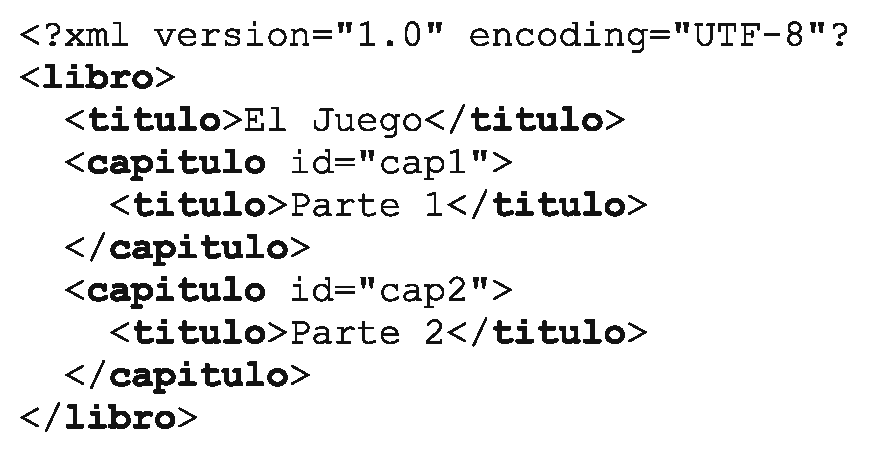
\includegraphics[scale=.5]{images/XML-document-example1}
%  \caption{\em Modelo de árbol para un documento XML.}
%  \label{fig:xml-tree-exa1}
%\end{figure}


\subsection{Historia de la impresión 3D}

El comienzo de la generación del concepto de impresión 3D puede ser rastreado al año 1976, a partir de la creación de la primera impresora a tinta por inyección \citep{maxey2013}. La utilización de la inyección de tinta abrió la pregunta respecto a qué tipo de materiales podían ser utilizados con esta tecnología, y cómo los mecanismos presentes en la época podían ser adaptados para abrir la posibilidad de ocupar otras materias primas. En Mayo de 1981, el Dr. Hideo Kodama del Instituto de Investigación Industrial del Municipio de Nagoya publicó detalles relativos a la técnica de prototipado rápido. Esta investigación se considera como la primera publicación que describe la técnica de fabricación capa a capa propia de los procesos de impresión 3D; no obstante, los desarrollos de Kodama no llegaron a ser materializados debido a problemas encontrados en el proceso de fundido de material. \citep{tresdsourced2020}. Paralelamente, la idea de ``máquinas de prototipado rápido'' continuó su desarrollo en Francia, por Jean-Claude André, Oliver de Witte y Alain le Méhauté. En la primera mitad de la década de los 80, le Méhauté investigaba en la empresa Alcatel sobre partes y piezas generadas a partir de la geometría fractal, y la manera en que éstas podrían ser fabricadas dada su complejidad de forma.
De Witte, quien era también investigador de Alcatel en el área de luz láser, propuso a le Méhauté que algunos líquidos compuestos por ciertos monómeros podían ser curados y transformados en sólidos tras la aplicación de luz láser, convirtiéndose en el primer paso para la construcción efectiva de máquinas de prototipado rápido a través de el proceso de Estereolitografía. Ambos compartieron el resultado de sus avances con André, que en ese tiempo trabajaba en el Centro Nacional Frances de Investigación Científica, para ya el año 1984 inscribir la patente de su desarrollo. Infortunadamente, el grupo debe abandonar el proyecto debido a problemas con la solidificación del material y poca rentabilidad desde la perspectiva económica \citep{alltresdp2018}.\

Con solo tres semanas de diferencia respecto a los investigadores franceses, Charles `Chuck' Hull solicita la patente del proceso de Esterolitografía con nuevos avances, como la utilización del formato STL (Standard Triangle Language) y la laminación digital de objetos. A diferencia del a Esterolitografía francesa, el método de Hull utiliza luz ultravioleta para el curado de fotopolímeros. El año 1986, obtenida su patente, Hull forma la empresa \textit{3D Systems} y lanza la primera impresora 3D, la \textit{SLA-1}, el año 1987 \citep{tresdsourced2020}.


\subsection{Métodos de impresión 3D}

\subsection{Impresoras 3D FDM}

\subsection{Tipologías de impresión 3D FDM}

\section{Mantenimiento}

\subsection{Historia y evolución del mantenimiento}

\subsection{Tipos de mantenimiento}

\subsection{GMAO}

\section{Lean Manufacturing}

\subsection{Historia Lean Manufacturing}

\subsection{Herramientas de mantenimiento}

\section{Design Thinking y Scrum}

\subsection{Metodologías ágiles}

\subsection{Scrum}

\subsection{Design Thinking}

\subsection{Fases del Design Thinking}

\subsection{Herramientas para diseño de Software}

\section{Desarrollo de Software}

\subsection{Programación orientada a objetos}

\subsection{Lenguajes de programación}

\subsection{Arquitectura Cliente-Servidor}

\subsection{API}

\subsection{Ordenadores de placa reducida}

 \ldots 

 

% Figura: \'Arbol XML 1
%\begin{figure}[tp]
%  \centering
%  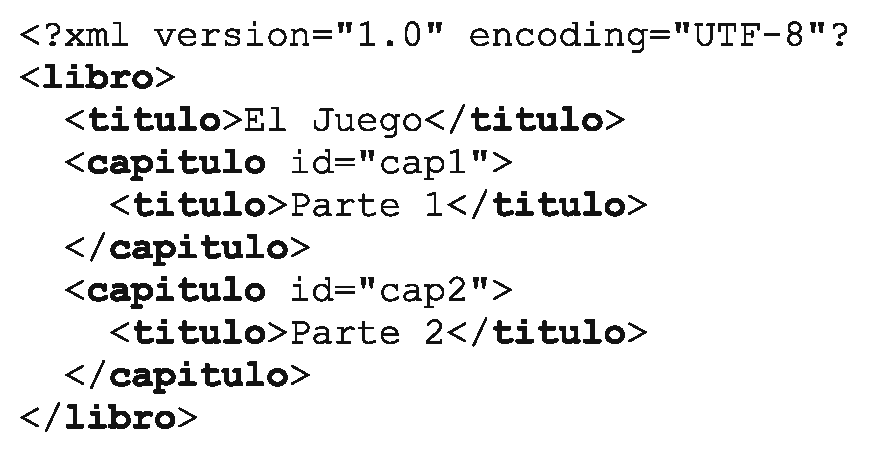
\includegraphics[scale=.5]{images/XML-document-example1}
%  \caption{\em Modelo de árbol para un documento XML.}
%  \label{fig:xml-tree-exa1}
%\end{figure}



